\part{"Jeune fille de province", "garçon" et "veuve d'âge mûr": une première approche socio-démographique des annonces}



\chapter{Femmes et hommes des petites annonces}

L'un des grands chantiers de l'historiographie du travail domestique à l'époque moderne a été d'établir le profil socio-démographique du groupe des travailleuses et travailleurs ancillaires, une tâche compliquée à la fois par la taille de ce groupe dans les grandes villes et leur présence très limitée dans les sources. Néanmoins, certains consensus existent: si la domesticité dans son ensemble est plutôt mixte, les employées de la "petite domesticité", qui concerne la grande majorité de la population, sont surtout des femmes, jeunes et non-mariées, souvent issues de la ruralité, et pour qui le statut de domestique est transitoire au moment de l'arrivée en ville. Ce profil ne doit cependant pas faire oublier la diversité interne à la domesticité, qui se manifeste notamment pour certains postes très particuliers car très qualifiés (secrétaires, hommes d'affaires, ...) ou dans les très grandes maisons. Dans ces cas, le genre du service tend à s'inverser et, de manière générale au XVIIIè siècle, plus on s'approche du haut de la hiérarchie ancillaire, plus la domesticité est masculine. Ainsi, Jacqueline Sabattier établit à partir du dépouillement d'insinuations testamentaires parisiennes de la fin du XVIIIè siècle que 54\% des domestiques sont des hommes, 46\% des femmes. Elle montre également que les femmes sont omniprésentes dans les maisons à moins de quatre domestiques, mais minoritaires et cantonnées aux rôles les moins rémunérés dans les maisons avec une domesticité importante. Par ailleurs, elle observe une augmentation de la petite domesticité féminine et une masculinisation croissante de la grande domesticité au cours du siècle; en clair, une division sexuée du travail de plus en plus marquée.

Qu'en est-il des domestiques des petites annonces? Dans quelle mesure les demandeurs et demandeuses d'emploi dans la presse correspondent-ils à cette démographie? Comment expliquer les éventuelles disparités entre ce groupe particulier et la population générale? À travers une analyse du sexe, de l'âge, de l'origine et de la situation déclarée des rédacteurs et rédactrices, il s'agit d'interroger la représentativité des annonces domestiques. 


\section{Méthode}

Après constitution du corpus, une première méthode exploratoire a consisté en la recherche basique des tokens "femme" et "homme" dans les textes, en vue d'obtenir un premier aperçu de la répartition genrée des annonces. Cette première méthode a permis d'extraire le genre de 2154 annonces (sur un total de 5064): 1451 hommes et 703 femmes. Évidemment, cette méthode comprend de nombreuses limites: elle ne prend pas en compte la diversité des qualificatifs employés dans les annonces (et qui sont particulièrement variés pour les femmes: fille, dame, veuve, demoiselle, ...). De plus, elle se base sur l'intégralité du texte de l'annonce, alors que les informations genrées sur le demandeur ou la demandeuse se concentrent au début de l'annonce; la présence du mot "homme" ou "femme" plus loin dans le texte n'est pas significative. 

\begin{figure}[h]
	\centering
	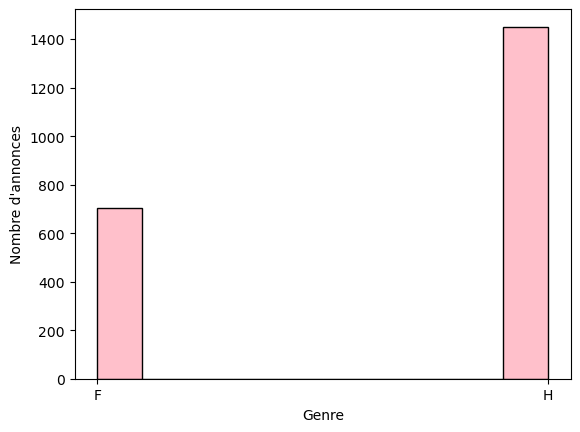
\includegraphics[width=12cm]{hist_genre_explo.png}
	\caption{Répartition des annonces selon le genre (méthode 1)}
\end{figure}


Ainsi, l'observation des limites de cette première méthode a mené à l'élaboration d'un script plus abouti pour extraire les informations liées au sexe de l'annonce: ce script sélectionne tout d'abord les cinq premiers mots de l'annonce (afin d'éviter la prise en compte de mots non significatifs, comme dans "un jeune homme de province, sans femme ni enfants"), avant d'extraire à l'aide d'expressions régulières certains qualificatifs de genre, dont la liste a été établie et amendée sur la base d'une lecture proche des annonces. Pour les annonces "masculines", ces qualificatifs sont: "homme", "garçon", "citoyen", "particulier", "sieur". Pour les femmes, il s'agit de : "femme", "fille", "dame", "demoiselle", "particulière", "veuve", "citoyenne". Les adjectifs "nommé" et "nommée" permettent d'inclure les annonces où les demandeuses et demandeurs sont appelés par leur nom ("Le nommé François..."). De plus, une dernière catégorie, "Personne", a été ajoutée pour les cas (nombreux) où l'annonce débute par "Une personne cherche..." ou, le plus souvent, "Une jeune personne cherche...". Si, dans le vocable du XVIIIè siècle, une "jeune personne" désigne plus souvent une jeune femme, j'ai tout de même préféré laisser ces cas de côté, en l'attente d'autres éléments de l'annonce qui permettraient de genrer celle-ci plus finement. 


\begin{table}[h]
	\centering
		\begin{tabular}{cclcc}
			\hline
			\textbf{Ville} & \textbf{Date} & \multicolumn{1}{c}{\textbf{Annonces}}                                                                                                                                                                                                                                                                        & \multicolumn{1}{c}{\textbf{Genre}} & \multicolumn{1}{c}{\textbf{Qualif. de genre}} \\ \hline
			Lyon           & 1802-10-09            & Une Veuve d'un âge mûr (...) & F                         & veuve                                      \\ 
			Lyon           & 1804-01-07        & Un Homme au fait du service (...)                                                                                                          & H                         & homme                                    \\ 
			Paris          & 1807-05-29      & Une personne âgée de 36 ans (...)                                                                                                        & Personne                  & personne                                  \\ \hline
		\end{tabular}
	\caption{Aperçu du \textit{dataframe} après extraction des informations genrées}
\end{table}

\section{Des annonces plutôt masculines, mais qui se féminisent lentement}

Avec cette deuxième méthode, il devient possible de définir le genre de 3611 annonces. Les annonces semblent demeurer en majorité écrites par des hommes:  1882 contiennent des qualificatifs masculins, contre 1045 pour les qualificatifs féminins. Néanmoins, l'hypothèse selon laquelle les annonces commençant par "une personne" (684 annonces) seraient plutôt féminines tendrait à relativiser ce constat et à rééquilibrer le \textit{sex ratio} du corpus. Les annonces dites "indéterminées" (c'est-à-dire celles pour lequelles on n'a pas pu aboutir à une classification femme ou homme) le sont pour diverses raisons: problèmes d'océrisation qui n'ont pas été corrigées ("Une jeune personné (sic) de 28 à 29 ans..."), problèmes de segmentation, usage de qualificatifs de métiers plutôt que de genre ("Un teneur de livres...", "Un jardinier...", "Deux frères..."). Enfin, cette approche ne fonctionne que dans les cas d'annonces de demandes d'emploi; les annonces d'employeurs, dont la forme est plus variée mais qui commencent souvent par "On desireroit trouver" ou "On cherche", nécessiteraient une autre méthode. 

Étant donné l'historiographie de la domesticité que j'ai évoquée plus haut, et selon laquelle femmes et hommes se répartissent différemment dans l'espace de la domesticité, ces résultats peuvent donner lieu à deux pistes d'interprétations. 
Première interprétation possible: les annonces sont plus employées par les hommes de manière générale, issus de la petite comme de la grande domesticité. La (légère) disparité entre annonces masculines et féminines s'expliquerait alors par un recours sexuellement différencié à ce support, qui pourrait s'expliquer de plusieurs façons: taux d'alphabétisation plus élevé pour les hommes au XVIIIè siècle \footcites{queniartEtapesResultatsProcessus1998} (bien que l'énonciation de l'annonce au Bureau d'adresses se fasse à l'oral, on peut supposer qu'il perdure un rapport différent à l'écrit), réseaux d'information différents quant à la recherche d'emploi. 
Deuxième interprétation: les annonces sont un support privilégié par la grande domesticité qualifiée, et délaissée, ou moins utilisée, par la petite et moyenne domesticité pourtant majoritaire dans la population générale, ce qui expliquerait ce déséquilibre. C'est l'hypothèse privilégiée par Ulrike Krampl qui, dans son dépouillement des\textit{ Affiches} entre 1760 et 1788, ne relève qu'un tiers d'annonces féminines\footcites{kramplPresseAnnoncesParisienne2020}.

\begin{figure}[h]
	\centering
	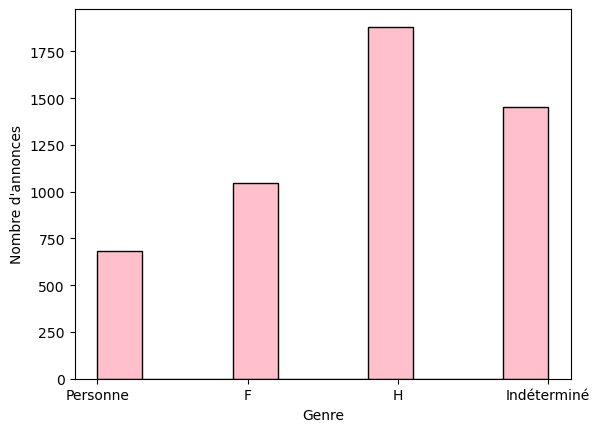
\includegraphics[width=12cm]{hist_genre.png}
	\caption{Répartition des annonces selon le genre (méthode 2)}
\end{figure}

En outre, l'analyse de la variable de genre dans le temps révèle un \textit{sex ratio} relativement stable: les annonces marquées comme masculines restent majoritaires des années 1750 jusqu'à la fin du siècle. Le changement le plus notable est l'apparition du qualificatif "personne" au début des années 1800 qui, si on l'interprète comme une marque du féminin, renverserait le genre des annonces en faveur des femmes: les annonces de femmes et de "jeunes personnes" constituent deux tiers des annonces d'emploi publiées en 1804, et près de trois quarts en 1807. Signe avant-coureur de la féminisation (ou de la démasculinisation) de la domesticité au XIXè siècle, hasard éditorial ou usage plus mixte du support de presse, qui se massifie durant cette période? Sans analyse des annonces sur une temporalité plus longue et avec un corpus plus exhaustif, il paraît difficile de conclure. 

\begin{figure}[h]
	\centering
	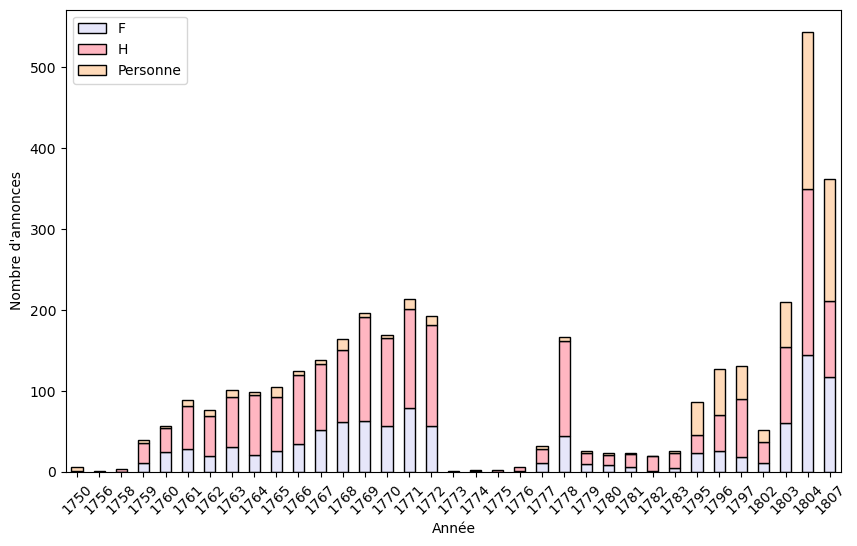
\includegraphics[width=12cm]{hist_genre_chrono.png}
	\caption{Répartition du genre des annonces dans le temps}
\end{figure}



\section{Des qualificatifs révélateurs du sexe mais également du statut social et matrimonial des demandeuses d'emploi}

Peut-être plus encore que la simple analyse sexuée des demandeurs d'emploi, l'analyse des mots employés dans les annonces pour désigner et donc assigner les individus à une catégorie sexuée est révélatrice du projet éditorial et du contexte politique de publication des \textit{Affiches}. Première observation: les qualificatifs féminins sont plus variés et révèlent davantage un statut social (d'âge, de matrimonie) que dans le cas des hommes. Là où les termes masculins emploient en grande majorité "homme" ou "garçon" (87\% des annonces d'hommes), les annonces féminines se répartissent entre "femme", "fille", "demoiselle", "mademoiselle", "dame" et "veuve". Ces qualificatifs renseignent non seulement sur le sexe de la demandeuse d'emploi, mais également sur son statut social et matrimonial, une information particulièrement importante pour les employeurs potentiels. En effet, si les hommes sont nombreux à être mariés parmi les domestiques du XVIIIè siècle, les femmes servantes représentent au contraire une population très majoritairement célibataire\footcites[p.79]{mazaServantsMastersEighteenthcentury1983}, et ce pour plusieurs raisons. Tout d'abord, la domesticité féminine est une condition souvent passagère, que les jeunes femmes exercent dans l'optique de se constituer une dot puis de s'établir. En outre, le célibat, ou en tout cas l'absence d'un mariage et d'une famille, est un critère d'employabilité important pour les femmes: si un homme marié peut continuer sans trop d'encombres à être valet, jockey ou régisseur, le mariage signifie immanquablement la fin du service domestique pour les femmes, notamment parce que les textes normatifs et législatifs de l'Ancien Régime réprouvent et stigmatisent l'emploi de servantes mariées\footcites[p.78]{mazaServantsMastersEighteenthcentury1983}. Dans ce contexte, la présence massive des qualificatifs "demoiselle" et "fille" dans les annonces peut être considérée comme une stratégie d'emploi, visant à se mettre en conformité avec l'idée que les maîtres et maîtresses se font de "la bonne domestique" au XVIIIè siècle.

Plus tard, la Révolution française introduit l'usage de "citoyen" et "citoyenne", termes à portée égalisatrice qui omettent volontairement la position sociale ou d'âge; c'est également le cas de "personne", dont l'usage augmente significativement à la fin du siècle (plus de 40\% des annonces publiées entre 1795 et 1807). Néanmoins, les lacunes du corpus dans les premières années révolutionnaires empêchent de véritablement mesurer leur apparition. 


\begin{table}[ht]
	\centering
		\begin{tabular}{lc}
			\hline
			\multicolumn{1}{c}{\textbf{Qualificatif de genre}} & \textbf{Occurrences} \\ \hline
			homme                                                & 1193            \\ 
			personne                                             & 684             \\ 
			garçon                                               & 448             \\ 
			fille                                                & 362             \\ 
			femme                                                & 258             \\ 
			(ma)demoiselle                                       & 211             \\ 
			particulier                                          & 187             \\ 
			veuve                                                & 128             \\ 
			dame                                                 & 74              \\ 
			sieur                                                & 26              \\ 
			citoyen                                              & 23              \\ 
			nommé                                                & 11              \\ 
			citoyenne                                            & 8               \\ 
			nommée                                               & 1               \\ \hline
		\end{tabular}
		\caption{Fréquence des différents qualificatifs sexués dans le corpus}
\end{table}


\begin{figure}[t]
	\centering
	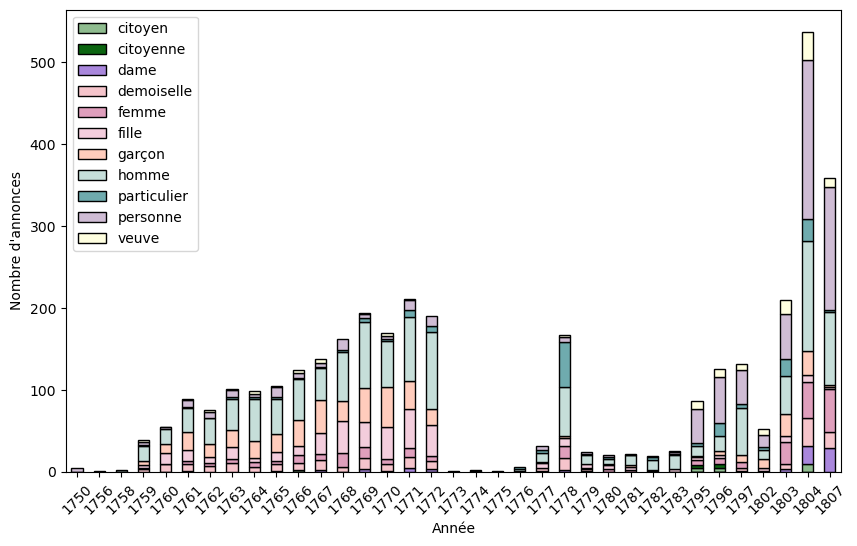
\includegraphics[width=12cm]{hist_qualif_genre_chrono.png}
	\caption{Répartition des qualificatifs sexués dans le temps}
\end{figure}



\chapter{La domesticité, une affaire de jeunesse?}

Si la domesticité concerne une part non négligeable de la population des trois villes étudiées, elle ne se répartit pas également dans l'espace social; l'un des apports de l'histoire démographique a notamment été de définir l'état ancillaire comme une étape du parcours de vie des individus, qui commence à l'adolescence et prend généralement fin avec le mariage, entre 25 et 30 ans au XVIIIè siècle\footcites{chamouxDomesticiteParcoursVie2009}. La condition domestique est donc majoritairement une condition de jeunesse, une condition transitoire censée attirer de très jeunes gens souhaitant s'établir en ville.

Qu'en est-il des petites annonces? Dans quelle mesure reflètent-elles cette réalité, ou s'en éloignent-elles? 



\section{Méthode}

Comme pour la variable de genre, l'extraction de l'âge des annonces s'est principalement faite sur la base d'expressions régulières. 

L'expression employée, \fbox{"(\textbackslash{w}+-?\textbackslash{w}*?) an(née)?s"} permet à la fois d'extraire les âges écrits en lettres ("vingt-quatre ans") et en chiffres ("32 années"). Puis, une librairie Python spécifique, text2num, a permis de transformer et d'harmoniser tous les résultats extraits en chiffres, afin de permettre des traitements quantitatifs. Cette méthode permet ainsi d'assigner un âge à 1256 annonces. 

Bien que ce nombre représente moins d'un tiers de annonces, cela ne signifie pas forcément que la méthode d'extraction est défectueuse; en effet, une lecture proche préalables des annonces a permis d'observer que l'âge est une information peu donnée par les domestiques. Plusieurs raisons peuvent expliquer cette absence: l'âge n'est pas (encore) un élément central de définition de l'individu à l'ère pré-statique, où l'enregistrement paroissial ou gouvernemental des naissances n'est pas généralisé\footcites{rennesAge2016}; il n'est pas rare de ne pas connaître son âge exact, et plusieurs annonces mentionnent d'ailleurs un âge approximatif ("autour de" ou "d'environ vingt-ans"). Avant le XIXè siècle, plus qu'un âge numérique exact, c'est surtout le positionnement dans un "âge de la vie" qui a cours\footcites{schmittInventionAnniversaire2007}: ainsi, la présence de qualificatifs ("jeune", "d'un âge mûr"...), moins précis mais qui pointent malgré tout vers une certaine période de l'existence, est commune dans les annonces. Certains exemples, qui cumulent position d'âge et de genre, ont déjà été évoqués (demoiselle, fille, garçon...). D'autres (jeunes, d'âge mûr, d'âge avancé, ...)ont pu être extraits à l'aide d'expressions régulières simples appliquées au début des annonces. Au final, 1391 annonces contiennent au moins un de ces qualificatifs;  la grande majorité (1066) contiennent l'adjectif "jeune". 
Si l'on comptabilise les annonces qui évoquent soit un âge numérique, soit un qualificatif d'âge, ce sont donc 1519 annonces qui contiennent une information relative à l'âge du demandeur ou de la demandeuse d'emploi.

Pour expliquer ce chiffre qui reste relativement bas, il faut envisager la possibilité que la mention de l'âge ne soit peut-être pas considérée comme un critère primordial de la recherche d'emploi, aussi bien pour les domestiques que pour les employeurs ou les rédacteurs du Bureau d'adresses. Si la jeunesse semble être une qualité valorisée, puisqu'une annonce sur cinq la mentionne, l'âge exact ou même imprécis ne semble pas être indispensable à l'embauche. Malgré ces éléments qui tendraient à relativiser l'importance de cette variable pour l'étude du corpus, que peut-elle nous apprendre sur la domesticité des \textit{Affiches}?


\section{Des annonces globalement jeunes, mais plus âgées que la norme domestique}

Les âges qui ont pu être extraits des annonces vont de 10 à 60 ans, mais sont très inégalement répartis: plus de 75\% des demandeurs et demandeuses ont entre 20 et 40 ans; l'usage des annonces semble assez limité pour les moins de 20 ans et les plus de 50 ans. Ces résultats vont dans le sens de la littérature et des données démographiques déjà évoquées: les jeunes adultes sont surreprésentés parmi la domesticité urbaine. 

Mais une observation plus fine de la répartition des âges permet de relativiser légèrement ce constat, et de noter une spécificité des annonces: la moyenne comme la médiane des âges se situe autour de 30 ans, ce qui est généralement donné comme la fourchette haute des âges de la domesticité (et correspond plutôt à l'âge du mariage); or ici, 50\% des demandeurs et demandeuses ont plus de 30 ans. Pratiquement autant d'annonces mentionnent un âge compris entre 20 et 30 ans (713 annonces) qu'un âge compris entre 30 et 40 (583). 

Plusieurs raisons pourraient expliquer cette (légère) différence d'âge entre domestiques en population générale et domestiques des annonces. Encore une fois, celles-ci pourraient attirer un profil particulier de domestiques, plutôt qualifié et plus âgé, la mention d'un âge plus avancé devenant alors synonyme non pas de vieillesse mais d'expérience. Autre hypothèse: l'annonce pourrait être envisagée comme support de recherche d'emploi alternatif par des individus qui ne correspondent plus au profil-type de la domesticité (très jeune, actif), et pour qui les réseaux habituels de recrutement ne suffisent plus. 


\begin{figure}[ht]
	\centering
	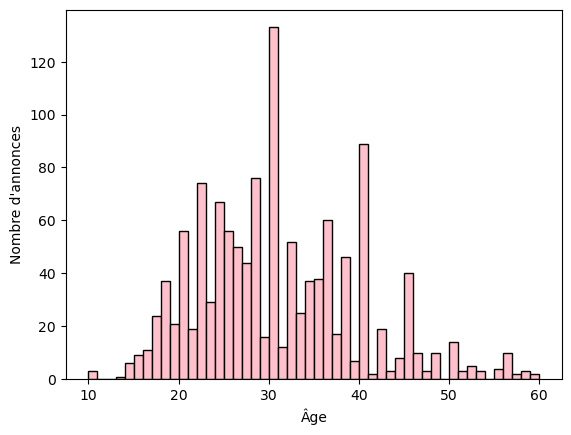
\includegraphics[width=12cm]{hist_age.png}
	\caption{Répartition des âges au sein des annonces}
\end{figure}

\begin{figure}[ht]
	\centering
	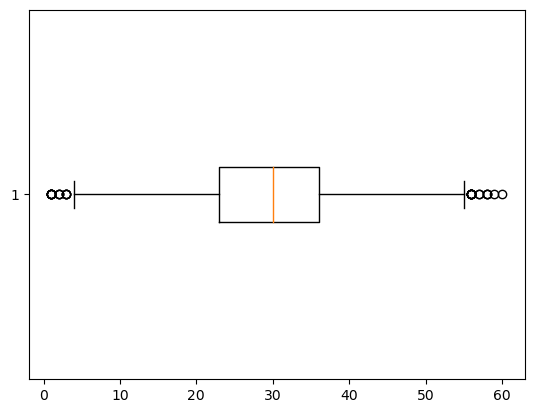
\includegraphics[width=6cm]{boxplot_age.png}
	\caption{Boîte à moustache des âges au sein des annonces}
\end{figure}



\section{Âge et genre des domestiques: des variables décorrélées}


Extraire l'âge  permet également de croiser cette information avec le genre des petites annonces. Dans la continuité de la littérature déjà évoquée, l'hypothèse la plus probable est celle de demandeuses d'emploi plus jeunes que leurs homologues masculins. 

Là-encore, néanmoins, les annonces révèlent une population distinctive, qui ne répondent pas au schéma d'une domesticité féminine jeune et d'une domesticité masculine au contraire plus âgée ou expérimentée. En effet, lorsqu'on isole les demandes féminines puis masculines, les moyennes et médianes demeurent autour de 30 ans; elles sont même légèrement plus élevés pour les femmes (autour de 32 ans), que pour les hommes. Le calcul d'un score de corrélation entre les deux variables donne un résultat très faible (-0.08), ce qui semble confirmer l'absence de relation statistique forte entre âge des genre des annonces. 

\begin{figure}[ht]
	\centering
	\begin{subfigure}[b]{0.4\textwidth}
		\centering
		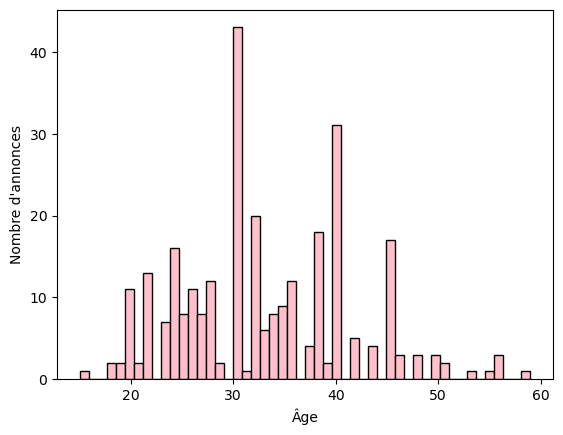
\includegraphics[width=6cm]{hist_age_F.png}
	\end{subfigure}
	\begin{subfigure}[b]{0.4\textwidth}
		\centering
		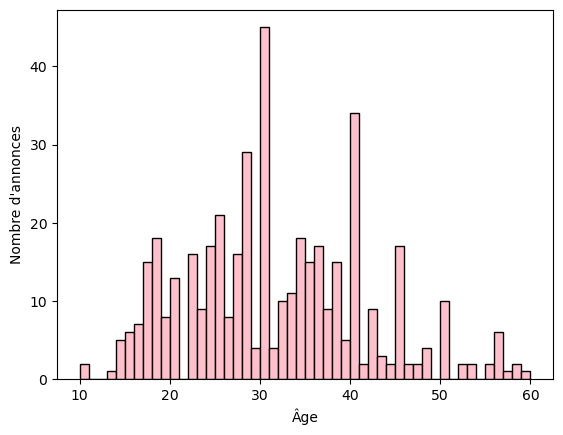
\includegraphics[width=6cm]{hist_age_H.png}
	\end{subfigure}
	\caption{Répartition des âges des annonces féminines (gauche) et masculines (droite)}
\end{figure}



En s'intéressant aux annonces qui contiennent à la fois ce qui parait être un qualificatif de sexe et d'âge ("fille", "garçon", "dame"...) et un âge numérique, on observe que ces qualificatifs ne semblent pas nécessairement refléter une position d'âge: les annonces qui contiennent les qualificatifs "garçon", "fille" et "demoiselle" ont les mêmes moyennes, médianes et répartition d'âge que l'ensemble. Ces derniers sont plus vraisemblablement des indicateurs de position ou de statut social, qui indiquent plutôt l'absence de mariage. La seule exception est le qualificatif "veuve": les demandeuses qui le mentionnent ont en moyenne 36 ans (médiane: 34 ans).



\chapter{"Arrivé des départements sans femme ni enfants": origines et situation des domestiques dans les annonces}

J'ai eu l'occasion dans les précédents chapitres de m'intéresser liminairement à la question de la position sociale et matrimoniale des demandeuses d'emploi. Cette variable, de même que l'âge et le sexe des domestiques, a beaucoup intéressé l'historiographie, qui s'accorde notamment sur l'importance du célibat au sein de la condition ancillaire \footcites{chamouxDomesticiteParcoursVie2009}. 

Un autre apport important de l'historiographie a été de mettre en évidence l'homogénéité de l'origine géographique et sociale du groupe domestique urbain: au XVIIIè comme au XVIIè ou au XVIè siècles, la grande majorité des domestiques ne sont pas originaires de la ville où ils travaillent. Jacqueline Sabattier, qui s'intéresse au cas de Paris, montre que trois domestiques de la capitale sur quatre viennent du Nord de la France, notamment de Normandie et de Picardie; parmi eux, quatre sur cinq sont issus de territoires ruraux. Parmi le reste, la majorité est née dans les campagnes périphériques du bassin parisien, ou dans des régions limitrophes (Bourgogne notamment)\footcites[p.20-25]{sabattierFigaroSonMaitre1984}. 

À partir de ces constats, que peuvent nous révéler les annonces à propos de la condition, de l'origine et du statut des domestiques? 


\section{Méthode}

Pour le statut matrimonial comme l'origine des annonces, la méthode employée a reposé principalement sur des recherches de mots-clés et d'expressions régulières dans le corpus. 

Concernant la situation matrimoniale, celle-ci n'étant pas signalé par des indices grammaticaux ou des constructions précises, j'ai constitué une liste d'expressions et de termes pouvant décrire différentes situations matrimoniales et familiales: "célibataire", "veuf" ou "veuve", "sans suite", "sans femme", "sans mari", "sans enfant", "marié(e)" ou "non marié(e). J'ai ensuite cherché ces termes dans les annonces, et les ai ajouté dans une nouvelle colonne du \textit{dataframe}.


Pour ce qui est de l'origine, j'ai extrait les ensembles de mots commençant par "arrivant de", "natif de" ou "venu de", ces expressions me semblant être les plus courantes dans le corpus pour signifier le pays ou la région de naissance des demandeurs et demandeuses. 

L'expression régulière obtenue est donc:

 \fbox{(?:arrivant | arrivée? |natif |native |venue? )(?:des |du |de )(?:(?i)\textbackslash w+)}, à partir de laquelle j'ai ajouté une nouvelle colonne au \textit{dataframe}. J'ai ensuite pu extraire plus précisément le lieu d'origine (ce qui suit "arrivant de..." donc), qui a donné lieu à une autre colonne. 


\section{Célibat domestique: la solitude comme argument de vente}

La recherche des mots-clés relatifs à la situation dans le corpus a permis d'extraire 501 annonces. Parmi elles, les qualificatifs qui se rapportent au célibat (sans enfants, sans suite...) sont très largement majoritaires (plus de 90\% des annonces extraites), notamment grâce à la présence importante de "veuve" dans le corpus (261 occurrences). 


\begin{table}[ht]
	\centering
	\begin{tabular}{lc}
		\hline
		\multicolumn{1}{c}{\textbf{Situation}} & \textbf{Occurrences} \\ \hline
		veuve                                            & 261                  \\
		veuve sans enfants                               & 72                   \\
		sans suite                                       & 46                   \\
		marié                                            & 36                   \\
		sans enfants                                     & 32                   \\
		veuve sans suite                                 & 15                   \\
		marié sans enfants                               & 10                   \\
		veuf                                             & 6                    \\
		célibataire                                      & 5                    \\
		sans femme sans enfants                          & 4                    \\
		non marié                                        & 4                    \\
		veuve célibataire                                & 3                    \\
		veuve sans enfants sans suite                    & 3                    \\
		mariée                                           & 2                    \\
		sans famille                                     & 1                    \\
		non mariée sans suite                            & 1                    \\ \hline
	\end{tabular}
	\caption{Répartition des qualificatifs de situation dans le corpus}
\end{table}

À partir d'un dixième du corpus, il est difficile de dire si les annonces sont représentatives de la population domestique générale. Néanmoins, cette omniprésence du célibat parmi les annonces qui mentionnent un statut matrimonial permet sans doute de confirmer la valorisation de la solitude domestique chez les employeurs: préciser qu'on est un ou une domestique seule, voire même insister sur cet aspect (en juxtaposant les expressions: "veuve sans enfants sans suite", "sans femme ni enfants", ...) n'a rien d'anodin dans un format de publicité de soi où chaque mot compte. 

Par ailleurs, l'observation des situations matrimoniales déclarées selon le sexe semble confirmer un acquis historiographique que j'ai déjà eu l'occasion d'évoquer: le célibat est plus valorisé (ou moins négociable) dans la domesticité féminine. Seules deux demandeuses disent être mariées, contre 46 demandeurs (dont dix "mariés sans enfants"). 

Enfin, il faut noter ici la représentation importante dans le corpus des veuves, proportionnelle à leur présence dans l'économie corporative ou domestique des villes françaises au XVIIIè siècle\footcites[p.5-18]{pellegrinVeufsVeuvesVeuvage2003}{lanzaVeuvesDansCorporations2009}.


\section{Des demandeurs principalement natifs des départements français}

La méthode employée a permis d'extraire l'origine de 71 annonces: 42 parisiennes, 27 lyonnaises et deux bordelaises. Un résultat décevant au regard de la taille du corpus, mais qui va dans le sens des observations faites lors des lectures proches des annonces: l'origine reste une information peu donnée par les domestiques. Cette absence s'explique peut-être par manque de place, ou parce que cette information est jugée peu pertinente, peu susceptible d'intéresser d'éventuels employeurs, voire dévalorisante. 

Néanmoins, les quelques dizaines d'origines qui ont pu être relevées donnent tout de même certaines informations, aussi bien relatives à la norme d'écriture des journaux qu'aux espaces et aux populations qui grossissent les rangs de la domesticité au XVIIIè siècle. Tout d'abord, l'observation des origines par ville révèlent des différences formelles importantes. Ainsi, les \textit{Affiches} de Paris emploient de manière massive l'expression, très générale, "des départements" ou "de son département", qui signifie qu'on vient d'une autre région que celle de la capitale; 30 annonces sur 42 l'utilisent. Le reste précisent des localités, souvent à l'étranger (Londres, la Suisse) ou restent plus vagues: "arrivant du Nord", "natif de province". 

Les\textit{ Affiches} de Lyon, au contraire, ont tendance à préciser le lieu d'origine: 15 annonces sur 27 mentionnent une localité précise, parmi lesquelles des villes et régions françaises proches de Lyon (Saint-Claude, Saint-Andéol-le-Château), plus éloignées (Paris,  Beaugency, Comtat, Franche-Comté, Mâcon) et des villes étrangères (Munich, Balten, Rome, Madrid). Le reste des annonces lyonnaises se répartit entre celles précisant venir "de cette Ville" (quatre annonces), "de la campagne" (deux annonces) ou de province (une annonce).

Les \textit{Affiches} de Bordeaux, si elles n'ont permis d'extraire que deux annonces contenant des origines, semblent suivre le modèle lyonnais, en indiquant précisément des localités (ici, Paris et Brest). 


Si cette méthode permet donc d'extraire en partie les origines des demandeurs et demandeuses et d'avoir un premier aperçu de la géographie de la condition domestique, elle est loin d'être exhaustive. Elle omet également le récit que certains domestiques font dans les annonces de leur parcours avant leur arrivée en ville, qui est un indicateur fort de la mobilité de travail sous l'Ancien Régime, comme par exemple dans cette annonce publiée à Lyon en mars 1770: "Un jeune homme de bonne famille, âgé de vingt ans, natif de Balten en Allemagne, qui a fait son apprentissage à Dijon, chez M. Foucherot; qui est d'un caractere doux, demande une place dans un Magasin de Draperie\footnote{\textit{Affiches de Lyon}, 29 mars 1770}". 



\bigskip

Ainsi, les annonces d'emploi, loin de pallier aux limites de la quantification de l'activité domestique, se heurtent finalement aux mêmes difficultés liées aux caractéristiques de l'ère pré-statique\footcites{fauve-chamouxSurplusUrbainFemmes1998} : des individus qui ne se définissent pas forcément par leur appartenance de sexe, encore plus rarement par leur âge. Des limites encore accentuées par la dimension déclarative des annonces, où se joue un enjeu de mise en valeur de soi, d'effacement et de dévoilement de l'information qui est bien éloignée des préoccupations de la démographie contemporaine.